%%%%%%%%%%%%%%%%%%%%%%%%%%%%%%%%%%%%%%%%%%%%%%%%%%%%%%%%%%%%%%%%%%%%%%
%%                     delay
%%%%%%%%%%%%%%%%%%%%%%%%%%%%%%%%%%%%%%%%%%%%%%%%%%%%%%%%%%%%%%%%%%%%%%

\subsection{Glyph: \glyph{delay}}\label{sec:delay}

The glyph \glyph{delay} is used to denote that the \glyph{activity node} linked as input does not produce the influence immediately.

\begin{glyphDescription}
 \glyphSboTerm SBO:0000225 ! delay.
 \glyphIncoming One \glyph{logic arc} (\sect{af:logicArc}).
 \glyphOutgoing  One \glyph{logic arc} (\sect{af:logicArc}) or one of the modulation arcs (\sect{af:arcs}).
 \glyphContainer A \glyph{delay} operator is represented by a circular shape containing the symbol ``$\uptau$`` (letter ``tau'' of the Greek alphabet).
The shape is linked to two ports, that are small arcs attached to the centres of opposite sides of the shape, as shown in \fig{af:delay}.
The incoming \glyph{logic arc} (\sect{af:logicArc}) is linked to the extremity of the leftmost or uppermost port, while the outgoing \glyph{logic arc} (\sect{af:logicArc}) or modulation arc (\sect{af:arcs}) is linked to the extremity of the rightmost or bottommost port.
 \glyphLabel None.
 \glyphAux None.
\end{glyphDescription}

\begin{figure}[H]
  \centering
  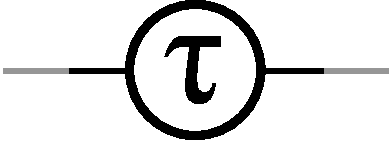
\includegraphics[scale = 0.6]{images/build/delay.pdf}
  \caption{The \AF glyph for \glyph{delay}.}
  \label{fig:af:delay}
\end{figure}
\normalcolor
